\documentclass[a4paper,10pt]{article}

%%Packages	%%%	%%%	%%%	%%%	%%%	%%%	%%%
\usepackage{amsmath,framed}
\usepackage[latin1]{inputenc} 	
\usepackage{listings}
\usepackage{xcolor}
\usepackage{graphicx}
\usepackage{placeins}

%%Settings	%%%	%%%	%%%	%%%	%%%	%%%	%%%
\renewcommand{\d}{\text{d}}
\newcommand{\e}{\text{e}}
\newcommand{\ve}{\mathbf}
\newcommand\numb{\addtocounter{equation}{1}\tag{\theequation}}

\setlength\fboxsep{1.2mm}
\setlength\fboxrule{0.5mm}


%%Margins	%%%	%%%	%%%	%%%	%%%	%%%	%%%
\usepackage{geometry}
\geometry{
  a4paper,
  left=35mm,
  right=35mm,
  top=25mm,
  bottom=25mm,
}

%%Header & Footer	%%%	%%%	%%%	%%%	%%%	%%%
\usepackage{fancyhdr}
\pagestyle{fancy}
\renewcommand{\headrulewidth}{1pt}
\rhead{Sara Danielsson, Mikael Perssson}
%8509080456 mitt persnr om vi vill ha det
\lhead{L3 DD2431}

\title{Lab 3, DD2431 Machine Learning}
\author{Sara Danielsson \\ Mikael Persson}
\begin{document}
%\maketitle

%\subsubsection*{Assignment 1}
\iffalse
Bayes Theorem is given by
\begin{align*}
  P(\alpha | D) &= \frac{P(D|\alpha)P(\alpha)}{P(D)} \Leftrightarrow \\
  \text{posterior} &= \frac{\text{likelihood}\times \text{prior}}{\text{evidence}},
\end{align*}
where $\alpha$ denote the model parameters and $D$ is the data.
\emph{Bayes Classification} uses the class posterior for a point $x^*$ belonging to a class
$k$ given by
\begin{equation*}
  P(k|x^*) = \frac{P_k(x^*|k)P(k)}{\underset{{k_i \in C}}{\sum}P_{k_i}(x^*|k_i)P(k_i)}
\end{equation*}
where $p_k(x^*|k)$ is the class conditional density, $C$ is the set of classes and $p(k)$
is the prior probability of class $k$. Assuming the density is described by a multivariat Gaussian 
we have
\begin{equation*}
  p_k(x|k) = \frac{1}{\sqrt{(2 \pi)^d \det \Sigma}}
  \e^{-\frac{1}{2}(x-\mu)\Sigma^{-1}(x - \mu)^\top}
\end{equation*}
where $x$ is a $1\times d$ row vector, and $\mu,\Sigma$ are the mean vector and 
covariance matrix respectively. Making the assumption that the data points are i.i.d. and 
maximizing the log likelihood gives the ML-estimates
\begin{align*}
  \mu_k &= \frac{1}{N_k}\sum_{i:c_i = k} x_i \\
  \Sigma_k &=
\end{align*}
\fi
\noindent
\textbf{Assignment 1}
\\
Please refer to the code for implementation of \texttt{mlParams()}.
Figure \ref{FIGas1} shows the result.




\FloatBarrier
\begin{figure}[h!]
  \center
  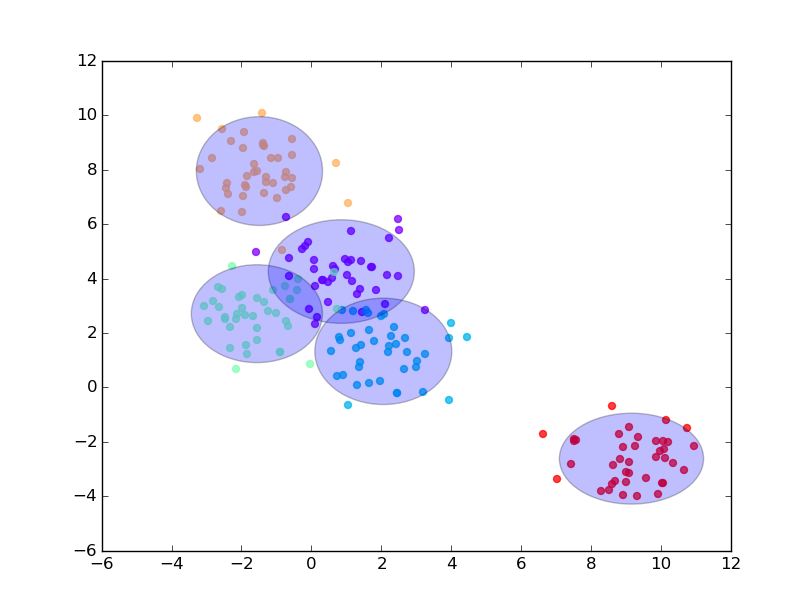
\includegraphics[width = 150mm]{figure_1.png}
  \vspace{-15mm}

  \begin{minipage}[t]{95mm}
    \caption{
      95 \% confidence intervals for data generated by \texttt{genBlobs(centers = 5)}
    }
    \label{FIGas1}
  \end{minipage}
\end{figure}

\FloatBarrier
$ $\\
\textbf{Assignment 2}
\\
Refer to code for implementations of \texttt{computePrior()} and \texttt{classifyBayes()}.



%\newpage
$ $\\
\textbf{Assignment 3}\\
The result of running \texttt{testClassifier(BayesClassifier(), dataset='iris', split=0.7)} and 
\texttt{testClassifier(BayesClassifier(), dataset='vowel', split=0.7)}
is given:
\begin{framed}
  \begin{scriptsize}
  \begin{verbatim}
  Trial: 0 Accuracy 84.4
  Trial: 10 Accuracy 95.6
  Trial: 20 Accuracy 93.3
  Trial: 30 Accuracy 86.7
  Trial: 40 Accuracy 88.9
  Trial: 50 Accuracy 91.1
  Trial: 60 Accuracy 86.7
  Trial: 70 Accuracy 91.1
  Trial: 80 Accuracy 86.7
  Trial: 90 Accuracy 91.1
  Final mean classification accuracy  89 with standard deviation 4.16
  Trial: 0 Accuracy 61
  Trial: 10 Accuracy 66.2
  Trial: 20 Accuracy 74
  Trial: 30 Accuracy 66.9
  Trial: 40 Accuracy 59.7
  Trial: 50 Accuracy 64.3
  Trial: 60 Accuracy 66.9
  Trial: 70 Accuracy 63.6
  Trial: 80 Accuracy 62.3
  Trial: 90 Accuracy 70.8
  Final mean classification accuracy  64.7 with standard deviation 4.03
  \end{verbatim}
  \end{scriptsize}
\end{framed}
\noindent
The decision boundary for the 2D-iris data is depicted in Figure \ref{FIGas2}.

\FloatBarrier
\begin{figure}[h!]
  \center
  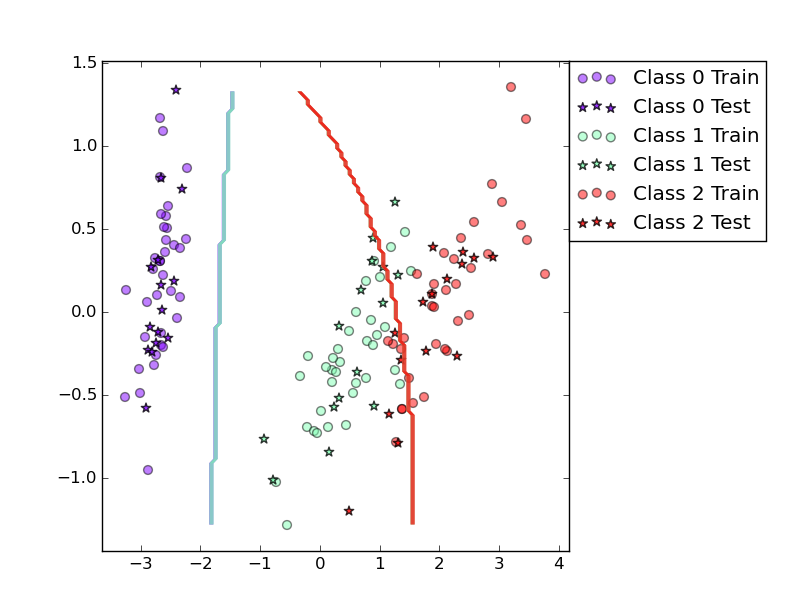
\includegraphics[width = 150mm]{figure_2.png}
  \vspace{-15mm}

  \begin{minipage}[t]{95mm}
    \caption{
      Boundary for the iris data.
    }
    \label{FIGas2}
  \end{minipage}
\end{figure}

\FloatBarrier
\noindent
Questions:
\begin{itemize}
  \item[1)] When can feature independence assumption be reasonable?
  \item[2)] How does the decision boundary look for the iris dataset? How could one improve the
    results for this scenario by changing the classifier, or by manipulating the data?
\end{itemize}
$ $\\
\textbf{Assignment 4}
\\
Refer to code for the augmented functions \texttt{mlParams()}





$ $\\
\textbf{Assignment 4}
\\






















\end{document}





